% Capítulo 6
\chapter{Estudo Experimental}
\label{cap:cap6}

Este capítulo consiste em apresentar o estudo, envolve a concepção de contexto do experimento, das configurações e características dos elementos envolvidos, a seleção das variáveis influenciadoras, o controle e a instrumentação do experimento, sua execução, a captura de dados durante experimentação, e por fim, a análise e conclusões obtidas a partir desses resultados. 

O objetivo do experimento é analisar a viabilidade do uso de mecanismos de \textit{throttling} como candidato para aumentar a disponibilidade dos elementos presentes em \textit{IoT} através do ajuste de comportamento por ação de limiares de atuação que consideram seus aspectos energéticos para assim,  prolongar a autonomia energética dos dispositivos. A abordagem é aderente e cobre os elementos presentes na taxonomia proposta no Capítulo \ref{cap:cap4} permitindo comparação e análise entre dispositivos que diferem sobre o fato de terem sua operação ajustada mediante \textit{throttling} ou não. 

\section{Metodologia}

O experimento pretende comparar os efeitos do mecanismo de \textit{throttling} em dispositivos com capacidade de coleta de energia, com foco em examinar a disponibilidade de cada um relacionada aos aspectos energéticos em condições de capacidade e atuação semelhantes.

\begin{figure}[H]
	\centering
	\caption{Etapas do Estudo Experimental.}
	\label{fig:cap6metodologia}
	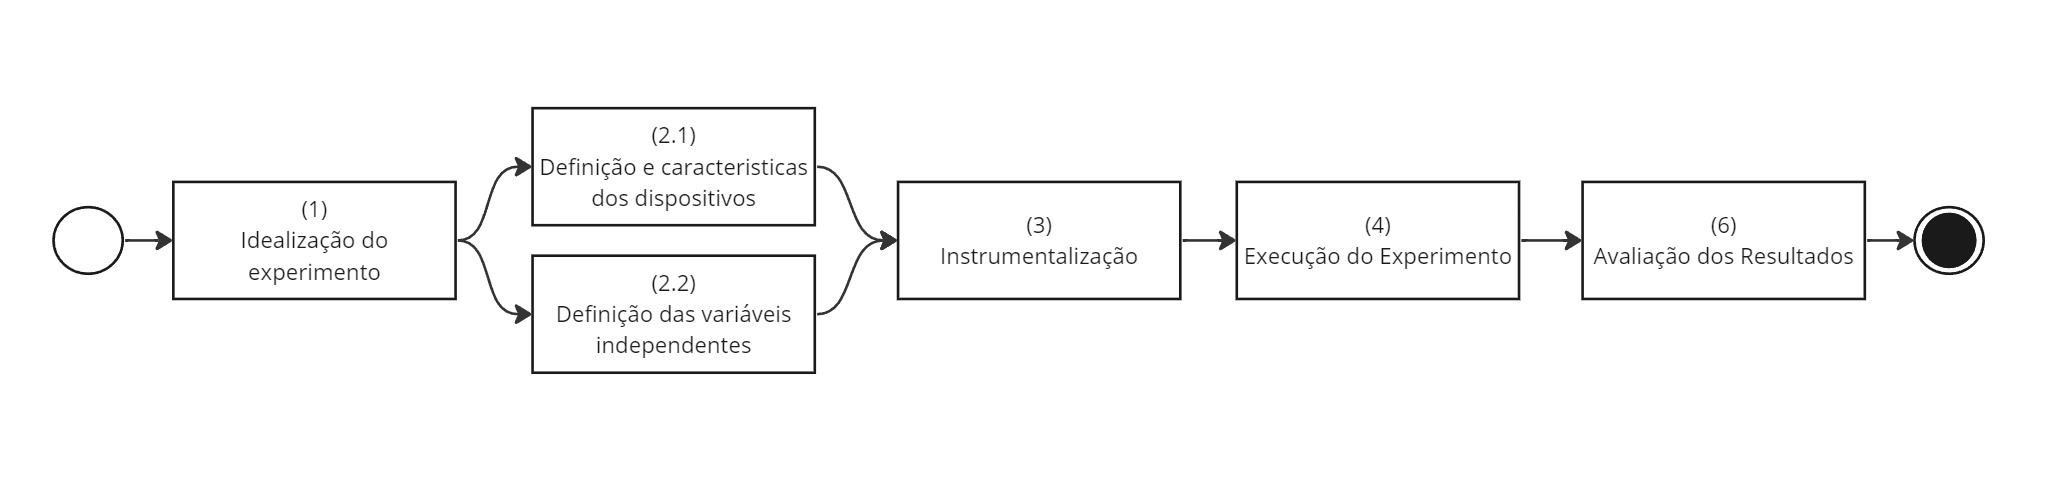
\includegraphics[width=1\linewidth]{Imagens/cap6/cap6metodologia.jpg}
	
	Fonte: elaborado pelo autor.
\end{figure} 

Para tal, buscou-se observar a influência do fator limitante na alteração do comportamento dos participantes em relação aos valores de energia coletada e reserva energética. Além disso, compreender sua eficiência na tomada de decisão em atender ou não às solicitações, em virtude da autoanálise de suas capacidades à medida que a variação de energia disponível ocorre. Este estudo visa analisar o uso de \textit{throttling} como possível solução para estender a disponibilidade de dispositivos com capacidade de coleta energética. 

A Figura \ref{fig:cap6metodologia} apresenta o fluxo de execução e ordem para as etapas realizadas. Na Seção \ref{cap6:idealizacao}, foi concebido quais os termos de projeto para viabilizar a análise e comparação de dispositivos com padrão \textit{throttling} aplicado as características energéticas, Etapa 1 - Idealização. Partindo daí, foi projetado ambiente para abstrair os elementos envolvidos, visando garantir equidade de condições e ações de maneira simultânea para todos os dispositivos durante a simulação. Para alcançar isolamento e consistência, optou-se pelo uso da plataforma Docker\footnote{O Docker é uma plataforma de virtualização que simplifica o desenvolvimento, envio e execução de aplicativos em contêineres. Disponível em \url{https://www.docker.com/}.} como agente facilitador, que atende às restrições necessárias de encapsulamento para que cada aplicação e suas dependências estejam contidas. 

A abordagem utilizando  \textit{containers} permitiu que os sistemas fossem estimulados simultaneamente, mantendo controle sobre recursos e garantindo os termos da operação: recursos energéticos e taxa de solicitações. Sendo assim, a composição do experimento considera que:  I - Dispositivos simulados com capacidade de coleta e armazenamento de energia estão inseridos em um dado ambiente semelhante ao uso real; II - Os dispositivos sempre recebem, ao mesmo tempo, um valor como coleta de energia; III - Os dispositivos participantes possuem a mesma capacidade para armazenar energia coletada; IV - Os dispositivos são submetidos simultaneamente aos mesmos ciclos de carga, compostos por uma quantidade fixa de solicitações.

Na Etapa 3 - Instrumentalização, capacita o experimento para capturar, apresentar e disponibilizar os resultados durante sua execução e posterior resumo dos dados obtidos, os detalhes estão descritos na Seção \ref{cap6:instrumentalizacao}. A Seção \ref{cap6:execucao} descreve os processos realizados na Etapa 4 - execução do experimento. Assim neste ponto, todas as etapas planejadas anteriormente ja estão implementadas. Em decorrência disso, habilita-se o experimento a executar seus procedimentos conforme um protocolo estabelecido, aplicando os estímulos já definidos (carga de solicitações e disponibilização de recursos energéticos) e coletando os resultados obtidos.

Ao final, a Seção \ref{cap6:avaliacao}, apresenta a avaliação dos resultados, que consiste na descrição e análise dos dados obtidos durante a execução. Os dados analisados são compostos pelo grupo de variáveis independentes que representam: Dos valores energéticos disponibilizados; da quantidade de solicitações realizadas. A análise se fundamenta em observar como o mecanismo \textit{throttling} implementado no dispositivo se colocará como agente atenuante do gasto energético utilizado a medida seus limiares de atuação são atingidos de acordo com o modo de operação previsto para determinados fatores observáveis presentes.

Ao fim da execução do experimento, as variáveis dependentes são obtidas para avaliação: a performance em relação a Quantidade total de solicitações atendidas ao fim da execução do experimento ea quantidade de solicitações impedidas mediante indisponibilidade de recursos em \textit{storage}. Ao aprofundar a análise, é preciso ainda, contrapor os dados temporais de oferta energética em relação a quantidade presente no dispositivo, o que justificará a atuação de limitadores e sua capacidade em manter um dispositivo operacional do ponto de vista energético.


\section{Idealização}
\label{cap6:idealizacao}
Uma vez definido os objetivos do experimento, a Etapa de idealização é o ponto onde foi construído as bases de execução do estudo. Assim, foram realizadas a estruturação  dos parâmetros e definição do cenário para realizar os testes, além da capacidade de coleta dos resultados e avaliação de conformidade com a taxonomia proposta.

O cenário foi idealizado para simular a atuação de dispositivos em dado um ambiente externo. Nele, provedores devem atender as solicitações de operações à medida que são providos energeticamente. Decorrente desta dinâmica, cabe ao provedor, com base nas condições energéticas, decidir se é capaz ou não de realizar a operação solicitada. Para atingir esse objetivo, o mecanismo de \textit{throttling} deverá atuar observando os recursos energéticos disponíveis.

Descreve-se \( C_a \) como o valor energético consumido pelo dispositivo quando estado ativo, \( C_i \), o consumo enquanto estado inativo e \( C_h \) representa dispositivos sem capacidade energética, com custo zero e portanto hibernando. Estima-se que, a duração de um ciclo $T(c)$ é obtida pela soma dos tempos onde o dispositivo esta ativo \( t_a \), que permanece inativo \( t_i \) e por fim o tempo que hiberna \( t_h \), possibilitando expressar o tempo total do ciclo em razão de $T(c_n) = $ \( t_a + t_i + t_h \).

O consumo total $C_{total}$, durante um ciclo é calculado com base em:
\[C_{total} = C_a \cdot t_a + C_i \cdot t_i + C_h \cdot t_h \quad (\text{Sendo }C_h = 0)\]
\[C_{total} = C_a \cdot t_a + C_i \cdot t_i\]
Considerando um dispositivo que permaneça ativo durante todo o ciclo \( t_a = T \), \( t_i = 0 \), \( t_h = 0 \):
\[ C_{total} = C_a \cdot T \]
De outra forma, caso permaneça hibernando durante todo o ciclo \( t_h = T \), teremos seu consumo total:
\[ C_{total} = C_t \cdot T = 0 \]
Assim, um dispositivo com ação do mecanismo \textit{throttling} deverá ter seu comportamento adequado ao modo de atuação projetado, através da recusa de solicitações, favorecendo manter-se em inatividade, cooperando para que reduza seu consumo durante um ciclo, assim conduz o dispositivo ao cenário onde \( t_a < T \) enquanto busca manter $t_h \approx 0$.

Ainda nesta etapa, foi necessário considerar uma configuração de componentes adequadas que pudessem representar minimamente um dispositivo com capacidade de coleta energética. Com esse objetivo, concebeu os aspectos de armazenamento (\textit{Storage}) e sua entrada energética simulando um valor coletado através de um \textit{Power Supply}. Assim, a dinâmica energética segue-se ao passo que um valor energético é apresentado em ciclos ao \textit{Storage}, que armazena e fornece os valores armazenados uso dos demais componentes presentes. A Figura \ref{fig:cap6dinamica} ilustra, a dinâmica energética de funcionamento do dispositivo.

\begin{figure}[H]
	\centering
	
	\caption{Dinâmica do fornecimento energético Dispositivo Provedor.}
	\label{fig:cap6dinamica}
	\noindent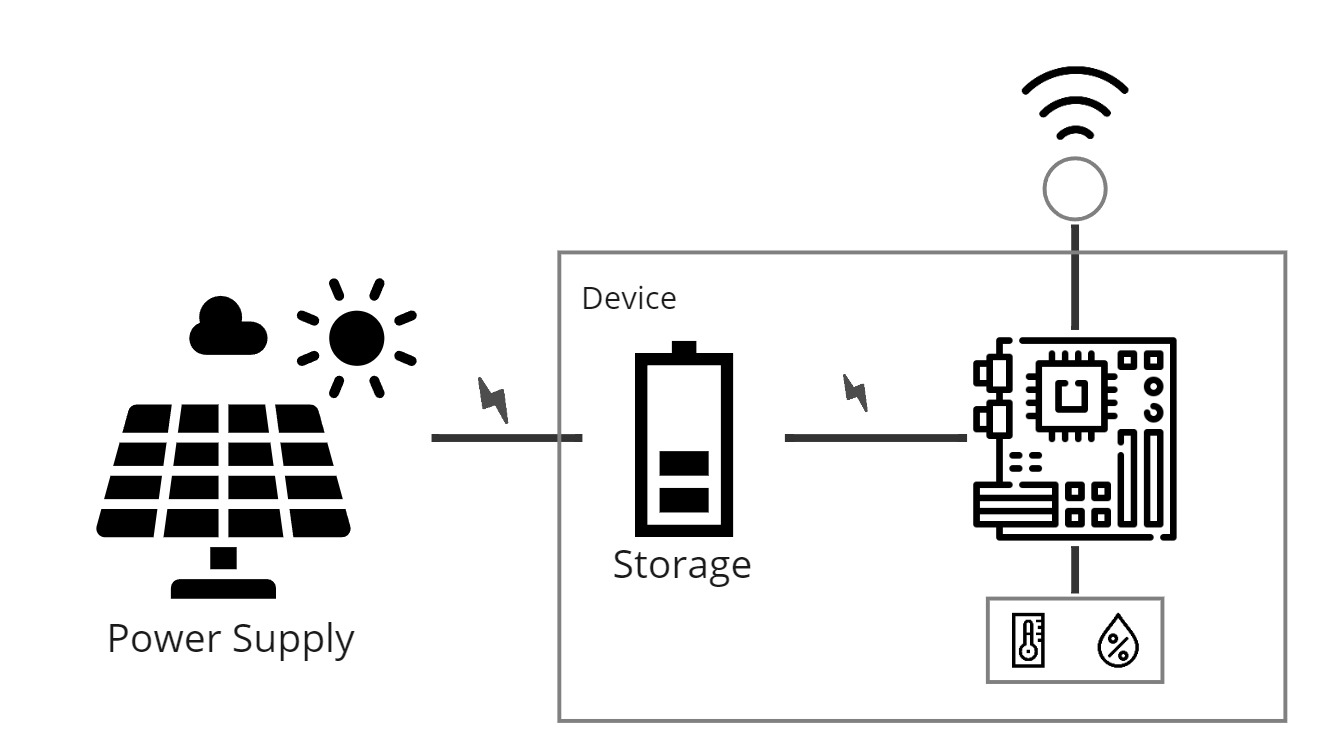
\includegraphics[width=0.75\linewidth]{Imagens/cap6/cap6dinamica.jpg} 
		
	Fonte: elaborado pelo autor.
\end{figure}


Em consequência, acontecendo disponibilidade energética, cabe ao dispositivo armazena-la a medida que os valores vão sendo apresentados. Paralelamente, os valores energéticos são disponibilizados na forma de recurso que deverá ser dispendido a medida que realiza as operações solicitadas.

Finalmente, o dispositivo deverá em todo seu funcionamento atuar dinamicamente em conformidade com os modo de operação projetados que representem os valores de recursos energéticos que possui. No experimento estão cobertos quatro modos de atuação a depender das capacidades energéticas:

\begin{enumerate}	
\item Modo Abundante: O Modo Abundante representa o dispositivo que possui recursos energéticos amplamente disponíveis, permitindo o funcionamento completo e otimizado de todas as suas funcionalidades. Aqui, atenderá quaisquer solicitação enviada, sem atuação do mecanismo limitante, aproveitando ao máximo a disponibilidade de energia;
\item Modo Atenção: Uma vez atingido este patamar, o dispositivo ainda apresenta condição energética razoável, porém moderadamente restringirá algumas operações atendidas com a motivação de preservar parte dos recursos até que um novo cenário energético seja apresentado;
\item Modo Alerta: É alcançado quando o dispositivo está operando com recursos energéticos extremamente limitados. Algumas operações ainda podem ser realizadas (conforme privilégios das operações ou solicitantes). Este modo motiva-se na intenção de prolongar a funcionalidade básica do dispositivo a todo custo enquanto tenta evitar a entrada no Modo Hibernação. 
\item Modo Hibernação: Este modo é ativado quando não possui mais recursos energéticos disponíveis para realizar operações. O dispositivo entrará em um estado de hibernação ou equivalente até que recursos energéticos sejam recuperados. Nenhuma ação de limitação acontecerá durante esse modo, caso hiberne,  o dispositivo encontra-se esgotado energeticamente.
\end{enumerate}

Um modo de operação representa como o mecanismo de \textit{throttling} agirá em detrimento do valor disposto em sua reserva energética, assim pode contribuir reduzindo a utilização dos recursos, amortizando ou interrompendo o uso energético nos serviços ofertados no dispositivo a medida que limita à capacidade de atendimento as solicitações. 

Naturalmente, os modos de operação podem sofrer variação, cabe a análise das especificidades e natureza que se destina cada implementação, para assim, dado o exame desses fatores que repousa na classe Meios da taxonomia Subseção \ref{cap4:atuacao_meios}, definir apropriadamente quais modos serão necessários para o dispositivo. Estes modos guiam a capacidade de mudança dos estados do dispositivo. Uma vez que, são justificados por tal modo a reduzir a quantidade de solicitações atendidas, proporcionando momentos em um estado de inatividade forçada contribuindo a utilização reduzida de recursos. De maneira geral, a dinâmica dos estados do dispositivo pode ser visualizada na Figura \ref{fig:cap6maquinaestados}. 

\begin{figure}[H]
	\centering
	
	\caption{Maquina de estados do Dispositivo.}
	\label{fig:cap6maquinaestados}
	\noindent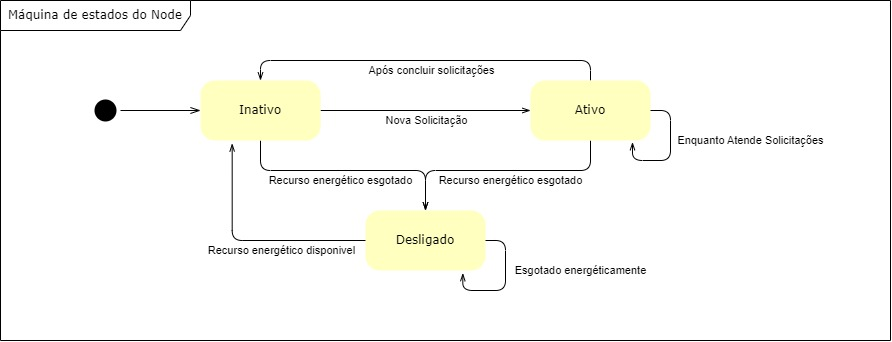
\includegraphics[width=0.75\linewidth]{Imagens/cap6/cap6maquinaestados.jpg} 
	
	Fonte: elaborado pelo autor.
\end{figure}

Por fim, os estados possíveis para o dispositivo são descritos como:
\begin{itemize}
	\item Estado Inativo: Aqui o dispositivo estará consumindo a menor quantidade de recurso energético possível. Enquanto inativo, encontra-se ocioso sem realizar nenhuma tarefa à medida que aguarda novas solicitações ou seja o caso necessário, aguarde nova entrada energética disponível, para atender solicitações anteriormente recusadas.
	\item Estado Ativo: Um dispositivo é considerado ativo enquanto atende solicitações. Nesse estado o dispositivo utilizará os recursos energéticos necessários para realização das atividades mediante o consumo desses recursos. 
	\item Estado Hibernando: No experimento, o estado hibernando é a indicação que o dispositivo não tem mais capacidade de assumir qualquer outro estado enquanto não receber recursos energéticos, seja por modo contundente de preservação ou em decorrência do esgotamento de suas reservas. Portanto, neste estado, um dispositivo não realizará qualquer atividade.	
	
\end{itemize}

A relação entre modos de operação e estados deixa implícita presença do mecanismo limitante e atuação implementada em cada modo, contribuindo para que o dispositivo permaneça em um estado de inatividade à depender das condições estabelecidas em que se encontra com a motivação de preservar ou restabelecer sua condição energética. Sendo assim, uma vez em determinado modo, o dispositivo terá uma quantidade potencial de atendimento das operações, estas, colocam o dispositivo em um estado ativo. Caso atinja valor limitador do modo, novas operações passam a ser negadas, e por sua vez, o dispositivo entrará em inatividade, reduzindo seu gasto energético.


\section{Definição das Variáveis Independentes e Dispositivos.}
\label{cap6:variaveisdispositivos}
A teoria de coleta de energia baseia-se na utilização de fontes energéticas disponíveis no ambiente para suprir, parcial ou totalmente, a demanda de um dispositivo inserido neste ambiente. Para o experimento, não há, a princípio, a intenção de analisar as particularidades para cada fonte energética, sua natureza e características de uso ou eficiência. 

Com isso, foi necessário para examinação e avaliação da aderência ao mecanismo de \textit{throttling} proposto abstração de fonte energética, uma vez que os recursos energéticos não seriam provenientes da dinâmica das condições de uma fonte qualquer. Quanto as possíveis novas implementações, ainda sim, caberá os ajustes necessários para atuação do \textit{throttling},  a depender da especificidade das condições submetidas ao dispositivo, assim como apresentado em \ref{cap:cap4} na classe Observáveis, esses aspectos são descritos como as questões relativas à entrada energética. 

Todavia, para a execução do experimento é necessário a compreensão sobre à disponibilidade e termos quantitativos de uma fonte de energia que represente valores de entrada para a coleta energética e assim utilizar esses dados como entrada para uma variável independente numérica. Sob tais restrições, os valores utilizados são semelhantes ao comportamento observado por um fonte de energia solar, para isto, seus valores foram concebidos com o auxilio dos dados disponibilizados no Atlas Brasileiro de Energia Solar \cite{martins2017atlas}. Particularmente, a definição dos valores de energia disponível orienta-se pelos parâmetros disponibilizados e apresentados para cidade de Natal/RN, nos termos da média diária de irradiação solar no decorrer  dos meses, o que rotulou-se uma Jornada $J_i$ (para $i = 1,2,...,12$). Os valores originários são expressos em  $Wh$, todavia para abstração criada a unidade de medida é utilizada apenas para manter a grandeza de comparação entre os ditos valores de consumo conforme Tabela \ref{table:cap6distribuicaonatal} onde cada valor representa o montante energético disponibilizado em uma respectiva jornada.

\begingroup

\setlength{\tabcolsep}{10pt} % Default value: 6pt
\renewcommand{\arraystretch}{1.5} % Default value: 1

\begin{table}[h]
	
	\centering
	\caption{Valores ofertados por ciclo}
	\smaller[8]
	\tabcolsep=0.05cm
\begin{tabular}{ c l | *{13}{c} }
	\toprule
	Jornada & $Wh$ & \multicolumn{13}{c}{Disponibilizado no Ciclo (c)}\\\cline{3-15}
	& & \begin{tabular}{@{}c@{}} c05 \\(0.007)\end{tabular} &
	\begin{tabular}{@{}c@{}} c06 \\(0.02) \end{tabular}	& 
	\begin{tabular}{@{}c@{}} c07 \\(0.053)\end{tabular} &
	\begin{tabular}{@{}c@{}} c08 \\(0.087) \end{tabular}&
	\begin{tabular}{@{}c@{}} c09 \\(0.105) \end{tabular}&
	\begin{tabular}{@{}c@{}} c10 \\(0.127) \end{tabular}& 
	\begin{tabular}{@{}c@{}} c11 \\(0.136) \end{tabular}& 
	\begin{tabular}{@{}c@{}} c12 \\(0.125) \end{tabular}& 
	\begin{tabular}{@{}c@{}} c13 \\(0.12) \end{tabular}& 
	\begin{tabular}{@{}c@{}} c14 \\(0.101) \end{tabular}& 
	\begin{tabular}{@{}c@{}} c15 \\(0.074)\end{tabular}& 
	\begin{tabular}{@{}c@{}} c16 \\(0.04)\end{tabular}&
	\begin{tabular}{@{}c@{}} c17 \\(0.005)\end{tabular}\\
	
	\hline
	J01 & 5674 & 39.72 & 113.48 & 300.72 & 493.64 & 595.77 & 720.6 & 771.66 & 709.25 & 680.88 & 573.07 & 419.88 & 226.96 & 28.37\\
	\hline
	J02 & 6017 & 42.12 & 120.34 & 318.9 & 523.48 & 631.78 & 764.16 & 818.31 & 752.12 & 722.04 & 607.72 & 445.26 & 240.68 & 30.09 \\
	\hline
	J03 & 6032 &  42.22 & 120.64 & 319.7 & 524.78 & 633.36 & 766.06 & 820.35 & 754.0 & 723.84 & 609.23 & 446.37 & 241.28 & 30.16 \\
	\hline
	J04 & 6082 & 42.57 & 121.64 & 322.35 & 529.13 & 638.61 & 772.41 & 827.15 & 760.25 & 729.84 & 614.28 & 450.07 & 243.28 & 30.41 \\
	\hline
	J05 & 5561 & 38.93 & 111.22 & 294.73 & 483.81 & 583.9 & 706.25 & 756.3 & 695.12 & 667.32 & 561.66 & 411.51 & 222.44 & 27.8\\
	\hline
	J06 & 5075 & 35.52 & 101.5 & 268.97 & 441.52 & 532.88 & 644.52 & 690.2 & 634.38 & 609.0 & 512.58 & 375.55 & 203.0 & 25.38 \\
	\hline
	J07 & 4658 & 32.61 & 93.16 & 246.87 & 405.25 & 489.09 & 591.57 & 633.49 & 582.25 & 558.96 & 470.46 & 344.69 & 186.32 & 23.29 \\
	\hline
	J08 & 4773 & 33.41 & 95.46 & 252.97 & 415.25 & 501.16 & 606.17 & 649.13 & 596.62 & 572.76 & 482.07 & 353.2 & 190.92 & 23.87\\
	\hline
	J09 & 5571 & 39.0 & 111.42 & 295.26 & 484.68 & 584.95 & 707.52 & 757.66 & 696.38 & 668.52 & 562.67 & 412.25 & 222.84 & 27.86\\
	\hline
	J10 & 5971 & 41.8 & 119.42 & 316.46 & 519.48 & 626.95 & 758.32 & 812.06 & 746.38 & 716.52 & 603.07 & 441.85 & 238.84 & 29.86 \\
	\hline
	J11 & 6112 & 42.78 & 122.24 & 323.94 & 531.74 & 641.76 & 776.22 & 831.23 & 764.0 & 733.44 & 617.31 & 452.29 & 244.48 & 30.56 \\
	\hline
	J12 & 6269 & 43.88 & 125.38 & 332.26 & 545.4 & 658.25 & 796.16 & 852.58 & 783.62 & 752.28 & 633.17 & 463.91 & 250.76 & 31.35 \\
\bottomrule
\end{tabular}
\label{table:cap6distribuicaonatal}
\\
\footnotesize Fonte: adaptado de \citeauthor{martins2017atlas}, (\citeyear{martins2017atlas})

\end{table}
\endgroup

O fator de distribuição atribuído a cada ciclo $c_i$ (para $i=0,1,2,...,23$) representa o aspecto da incidência solar em  dado instante $i$ em relação ao total esperado para uma jornada $J$ (na totalidade dos 24 ciclos). Para atribuição dos pesos dispostos, foi utilizada a referencia disponibilizada em \citeonline{tutiempo2023} para o dia 12 de dezembro de 2023. Aqui destaca-se que a limitação de adotar a distribuição solar para um dia especifico é justificada pela intenção de apenas conceber os valores capazes de cobrir o objetivo do experimento, a medida que aparentemente aproxima-se de termos que caracterizam fonte energética solar. 

Sendo assim, obteve-se a valoração das quantidades ofertadas como entrada energética, em referencia as jornadas aplicados aos fatores de incidência encontrados em cada ciclo. Finalmente, os ciclos $c_0, c_1,... c_4$ e $c_{18}, c_{19},... c_{23}$ possuem peso atribuído nulo, representam ciclos onde não existe energia coletável significante, em conformidade com a referencia solar e suas características utilizadas, motivo para estarem suprimidas na Tabela \ref{table:cap6distribuicaonatal}.

Os valores de cada ciclo são ofertados como estimulo ao dispositivo provedor no decorrer do experimento, e ao fim do ciclo $c_{23}$ de uma dada jornada $J_i$, inicia-se jornada $J_{i+1}$ seguinte até que todos os ciclos presentes nas em 12 sejam ofertadas. Esta abordagem garante que todos os cenários previstos para o experimento são cobertos em sua execução e possibilita a geração e analise dos resultados obtidos.

Com a definição dos ciclos e jornadas, determina-se também como acontecerá os processos de oferta energética. Partindo disso, surge a necessidade para definir como se dará o processo de utilização desses recursos já armazenados. Uma segunda variável independente é necessária, o objetivo é realizar solicitações ao dispositivo de modo a estimular demanda ao mesmo. Assim, é preciso adotar algumas práticas para garantir que todos os dispositivos, além de receber a oferta energética estipulada como projetado, também sejam capazes de receber a mesma carga de solicitações, aproximadamente ao mesmo tempo. 

Ao atender uma solicitação, o dispositivo é conduzido para ingressar ou permanecer em estado ativo, este intensifica a utilização de recursos quando comparado com um estado inativo ou enquanto hiberna, conforme mencionado na Seção \ref{cap6:idealizacao}. Para cobrir essa dinâmica, após os dispositivos recebem a primeira oferta energética, no inicio da execução do experimento, a partir daí, serão solicitados simultaneamente aos dispositivos 5 solicitações por segundo. na razão aproximada de 1 solicitação a cada 0.2 segundos. Caso dispositivo não consiga receber uma solicitação, na janela de tempo, será considerado indisponível para aquele estimulo. 

Considera-se que os termos necessários para transmissão ou as características da interface de comunicação podem exercer influência na razão de transmissão das solicitações, por este motivo é previsto que dada a quantidade total de solicitações realizadas possam ter pequena variação ao fim da execução do experimento. Em todo caso, é garantido em que todos os dispositivos foram estimulados ao mesmo valor total de solicitações bem como foram solicitadas simultaneamente.

Finalmente, esta variável independente numérica, solicitações realizadas, carrega os valores totais de requisições, em decorrência dela, observa-se os valores encontrados para a quantidade total de solicitações atendidas e o total de solicitações realizadas que encontraram o dispositivo indisponível. 


\subsection{Dispositivos}

Foi construído um modelo capaz de representar um dispositivo sensor embarcado com os mecanismos do \textit{throttling}, este dispositivo é uma abstração que deverá receber estímulos como entradas energéticas em um cenário simulado, a medida que utiliza esses recursos para atender solicitações continuas em uam interface de acesso provisionada. A visão geral do dispositivo provedor e componentes pode ser visto na Figura \ref{fig:cap6providernode}. Além disso, o código fonte do mesmo está disponível no repositório Git\footnote{Código-Fonte do dispositivo provedor em \url{https://github.com/eusoupaulolopes/mst_experiments}.}  para análise e colaboração.

\begin{figure}[H]
	\centering
	
	\caption{Componentes do dispositivo Provedor.}
	\label{fig:cap6providernode}
	\noindent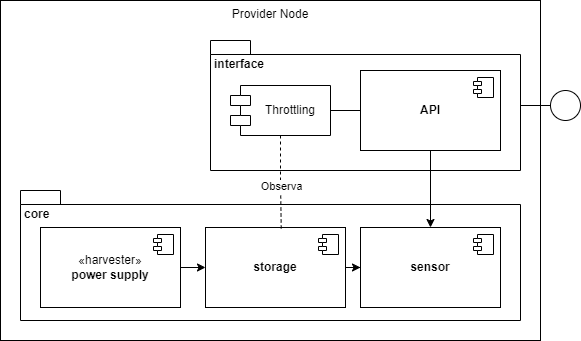
\includegraphics[width=0.75\linewidth]{Imagens/cap6/cap6providernode.png} 
	
	Fonte: elaborado pelo autor.
\end{figure}

Os elementos idealizados que constituem o dispositivo provedor são referentes aos seguintes componentes:
\begin{enumerate}
	\item \textit{Power Supply}, é responsável por fornecer a energia necessária para o funcionamento do dispositivo, simulando a coleta de energia de acordo com os ciclos descritos na Tabela \ref{table:cap6distribuicaonatal}. O componente atuará em paralelo a outras atividades realizadas. Caso o armazenamento do dispositivo esteja completamente cheio, ainda assim os valores de entrada serão entregues, representando desperdício energético. O esgotamento energético do dispositivo não representa a incapacidade de receber novas entradas energéticas e com isso, assumir novos estados de operação.  
	
	\item \textit{Storage}, responsável por armazenar os valores energéticos oferecidos mediante sua capacidade e a partir disso, oferecer a energia coletada, sendo um componente suplementar com o objetivo de manter disponibilidade energética do dispositivo sob certas circunstancias. A capacidade definida para o \textit{storage} do dispositivo provedor pode ser ajustada e deve representar a aderência da configuração proposta para um \textit{buffer} energético no cenário de uso.
	
	 \item \textit{Sensor}, cabe a este componente simular as atividades executadas pelo dispositivo. Dentre as características presentes em Sensor, esta a indicação do gasto energético momentâneo mediante o estado que se encontra em referencia aos possíveis estados já apresentados na Figura \ref{fig:cap6maquinaestados}. Assim, é possível configurar um dispositivo para embarcar um ou mais sensores, mediante implementação da especificação de seus custos energéticos operacionais em cada estado possível. Assim, o dispositivo é capaz de simular um ou mais sensores diversos, temperatura, umidade, pressão, luminosidade, presença, entre outros, caso necessário.
	 
	 \item \textit{Interface} é o ponto de entrada para recebimento das solicitações de sensoriamento, componente de interação com o dispositivo. O mecanismo de \textit{throttling} atuará acoplado a interface provida, controlando a vazão de atendimento a medida que permite ou bloqueia as solicitações recebidas em garantia de manter o modo de operação em sincronismo ao estado das suas capacidades energéticas. Assim, uma vez atingido um limiar observado, instantaneamente o dispositivo poderá negar novas solicitações ainda na interface, impedindo assim a propagação da mensagem que estimularia o seu grupo de sensores para atender a demanda solicitada, e através disso amortizando o gasto energético total do dispositivo.
	 
\end{enumerate}


\section{Instrumentalização.}
\label{cap6:instrumentalizacao}
Os processos executados para instrumentalização foram fundamentais para garantir a precisão e confiabilidade dos dados gerados durante a execução do experimento. Para isso, foram utilizadas algumas soluções e o processo de decisão e escolha entre as ferramentas se deu com base na adequação à necessidade especifica do experimento realizado. Além de cobrir os aspectos de coleta dos dados de forma objetiva, também foi essencial para os critérios de visualização e análise dos resultados.

O processo de coleta dos dados deve acontecer em intervalos regulares de 10 segundos definidos no plano experimental, assim, todos os dados gerados são coletados simultaneamente em todos dispositivos. Cabe também a necessidade de armazenamento dos dados capturados para análise, que pode acontecer sincronizadamente durante execução ou em momento posterior. Para isso, justifica-se a preferencia de uso por uma ferramenta de uso livre, que fosse capaz de agregar em sua estrutura operacional aspectos para coleta de dados, armazenamento e consultas. A solução Prometheus\footnote{Disponível em \url{https://prometheus.io/}.}, foi capaz de atender os pontos elencados, alem de ser aderente a estrutura criada para execução do experimento.

Para tanto, de maneira transparente é embarcado no dispositivo um cliente Prometheus chamado \textit{Exporter}, este é responsável por expor os dados observáveis e de interesse no dispositivo. Periodicamente, a cada 10 segundos, um agente externo Prometheus \textit{Collector} irá realizar chamadas com o objetivo de capturar os dados expostos pelo \textit{Exporter}. Assim, durante atividade de coleta, cabe ao agente coletor as ações de solicitar os dados providos no cliente para conversão e armazenamento destes na forma de séries temporal. 

Todos os dados recuperados pelo coletor são disponibilizados e mantidos em uma estrutura temporal no serviço Prometheus. Graças a essa estrutura, qualquer visualizador capaz de realizar consultas em um formato PromQL - \textit{Prometheus Query Language} estará habilitado para acompanhar execuções em andamento. A Figura \ref{fig:cap6instrumentalizacao} ilustra a dinâmica entre dispositivos e seus \textit{Exporters} embarcados e o agente externo coletor, e, por consequência, a disponibilidade dos dados para uma \textit{dashboard} de acompanhamento e posterior análise dos resultados. 

\begin{figure}[H]
	\centering
	
	\caption{Coleta e visualização da Execução do Experimento.}
	\label{fig:cap6instrumentalizacao}
	\noindent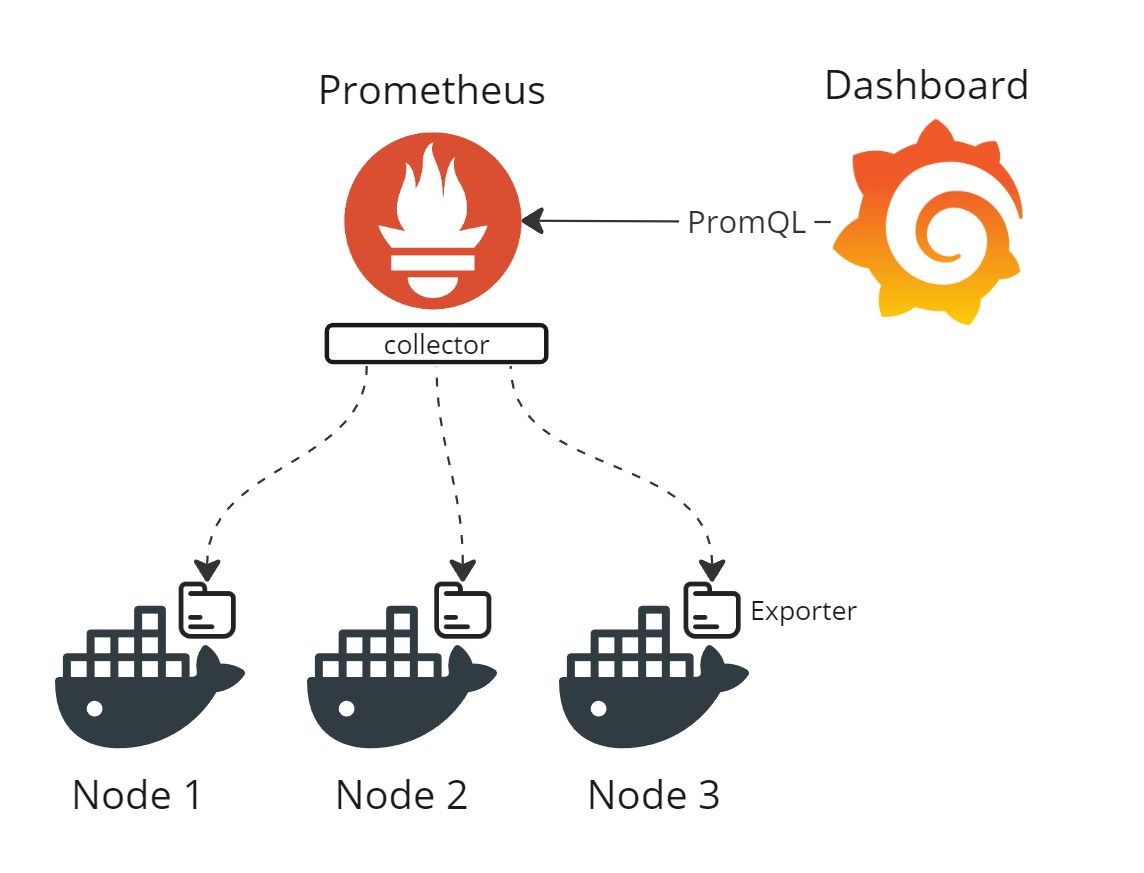
\includegraphics[width=0.75\linewidth]{Imagens/cap6/cap6instrumentalizacao.jpg} 
	
	Fonte: elaborado pelo autor.
\end{figure}


Com a necessidade de visualização dos dados durante execução, foi criado uma \textit{dashboard}  para apresentar os resultados obtidos de forma gráfica. Logo, com o auxilio da ferramenta Grafana, uma plataforma de análise e visualização de dados através de quadros - \textit{dashboards} personalizáveis, foi criado a interface de acompanhamento do experimento. a Figura \ref{fig:cap6bashboard} apresenta o configuração da interface criada. Para avaliação  posterior após a execução do experimento, os dados foram coletados através os logs gerados, e submetidos a uma planilha eletrônica capaz de produzir os gráficos necessários para análise dos resultados. 

\begin{figure}[H]
	\centering
	
	\caption{Dashboard para visualização dos resultados.}
	\label{fig:cap6bashboard}
	\noindent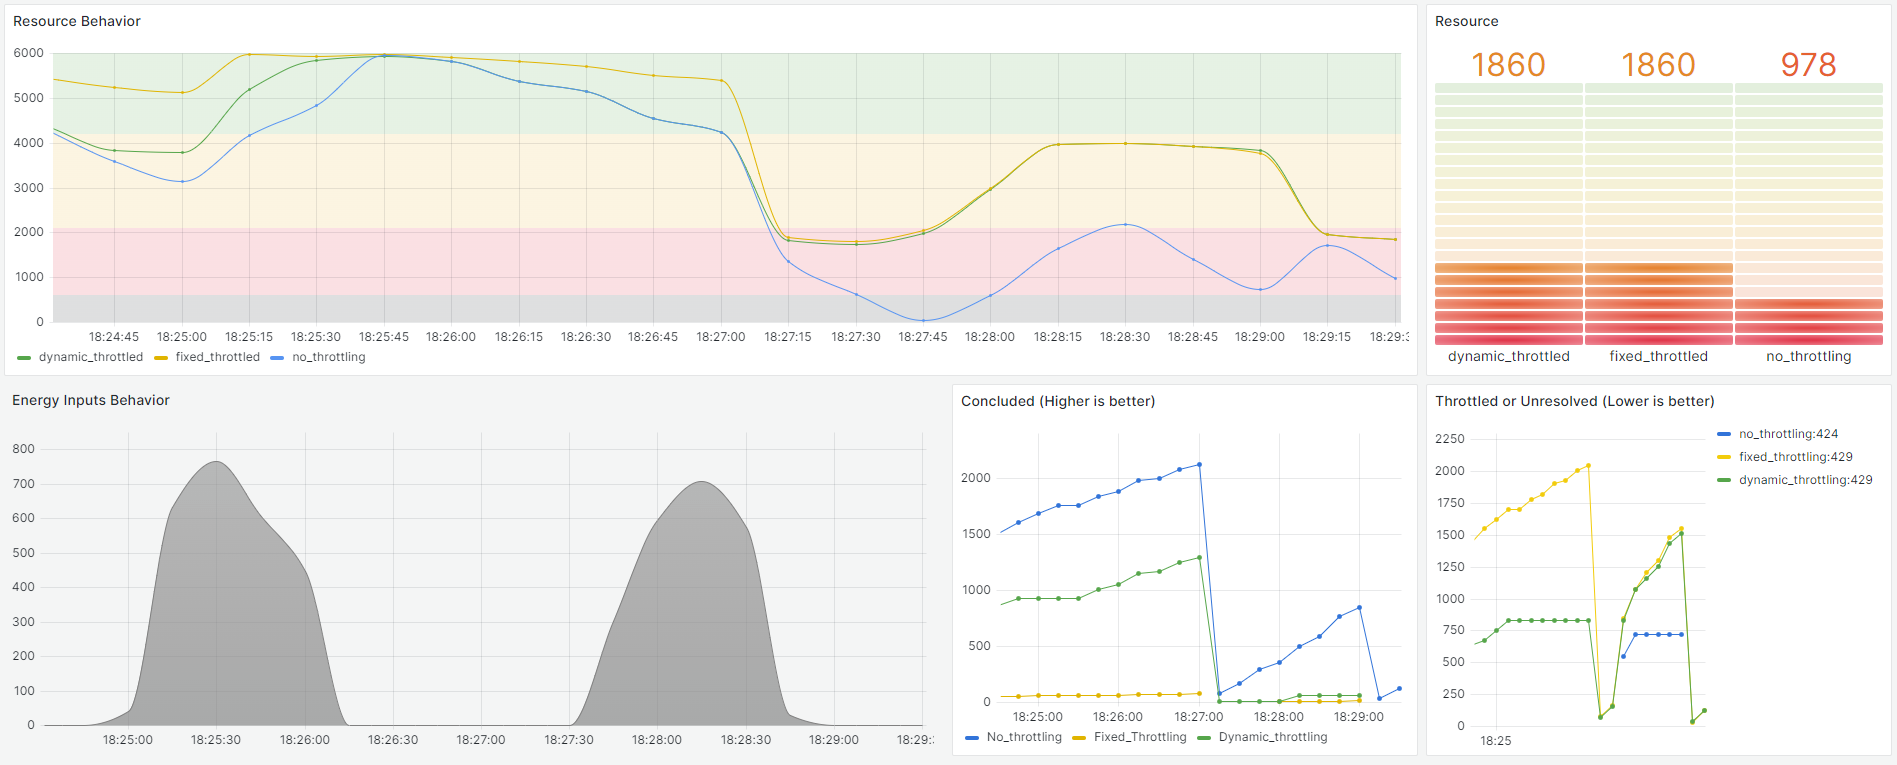
\includegraphics[width=1\linewidth]{Imagens/cap6/cap6dashboard.png} 
	
	Fonte: elaborado pelo autor.
\end{figure}

É pertinente ressaltar que os processos realizados para instrumentalização, em especial o \textit{Exporter}, não deve exercer influência sobre a gasto energético simulado do dispositivo durante execução do experimento. Seu uso e custos são transparentes para a implementação, funcionando como um agente independente que não interfere nas dinâmicas energéticas colocadas em análise.

\section{Execução.}
\label{cap6:execucao}

As execuções foram conduzidas para garantir a confiabilidade e relevância do experimento e resultados obtidos. O estudo experimental foi realizado em etapas conforme descritos em referencia a Figura \ref{fig:cap6metodologia}, As variáveis independentes utilizadas foram controladas para minimizar possíveis viés e garantir a consistência e replicabilidade do experimento. Durante a execução, os processos de instrumentalização atuaram em conformidade para que enquanto os dados necessários eram coletados, nenhuma variável externa pudesse influenciar nos resultados.


No inicio de uma execução, o valor atribuído como reserva energética disponível no \textit{Storage} é equivalente a sua capacidade máxima de armazenamento, a partir disso, os valores de entradas energéticas disponibilizadas pelo \textit{Power Supply} seguem a referencia apresentada na Tabela \ref{table:cap6distribuicaonatal}, submetidos a medida que se inicia um novo ciclo $c_0, c_1,...,c_{23}$ relativos cada jornada $J_1, J_2, ..., J_{12}$. Dado controle do experimento, a execução atende as características gerais com certa previsibilidade e após 3 execuções, foram identificados os valores conforme descrito na Tabela \ref{table:cap6:execucaocaracteristicas}.


Portanto, ao iniciar um ciclo $c_n$, o valor de entrada energética referente é entregue e, por sua vez, armazenado em componente adequado, passados 6 segundos previstos, um novo ciclo $c_{n1}$ inicia-se encerrando o anterior mediante uma nova entrada energética disponibilizada. Este processo, de ativar todos os ciclos de todas as jornadas acontece em em 1728 segundos totais, tempo necessário para que o experimento apresente a atuação completa da dinâmica de estados e modos de operação possíveis.

Apoiado nisso, as solicitações requeridas são disparadas contra os dispositivos durante os ciclos $c$. Assim, ininterruptamente, todas solicitações devem ser atendidas caso dispositivo esteja em modo semelhante ao abundante. Para isto, três simulações foram utilizadas, a referencia das características são encontradas na Tabela \ref{table:cap6:dispositivosutilizados} e indicam a composição dos dispositivos simulados respeito as classes taxonômicas de Atuação do mecanismo \textit{throttling}. 


\begingroup


O dispositivo disp$_1$, representa o comportamento de dispositivos sem nenhum mecanismo de limitação das solicitações, seu objetivo é servir como base de comparação para o consumo energético a medida que deverá atender todas as demandas solicitadas enquanto não se encontrar em estado hibernando.

Por sua vez, disp$_2$  e disp$_3$ foram implementados com a capacidade de limitar suas operações. Entretanto a atuação do mecanismo \textit{throttling} é distinta entre eles, para o disp$_2$ é realizada restrição mediante limiar fixado em razão de uma vazão de atendimento estipulada previamente sem observar adequação ao cenário energético. Já para o disp$_3$ o limiar irá atuar adaptativamente regulando a taxa de vazão de atendimento observando as condições de sua Reserva energética.

\begin{table}[htbp]
	
	\centering
	\caption{Instancia taxonômica para os dispositivos.}
	\small
	%	\tabcolsep=0.05cm
	\begin{tabular}{ c c c c c c c}
		\toprule
		Dispositivo & Nome & \textit{Throttling} & \multicolumn{4}{c}{Atuação}\\\cline{4-7}		
		& & & Limiar & Ciclos & Meios & Observáveis\\
		\midrule
		%		\hline
		disp$_1$ & no-throttling  & Não & - & 288 & - & - \\
		disp$_2$ & fixed-throttling  & Sim & Fixo & 288 & Vazão & - \\
		disp$_3$ & dynamic-throttling  & Sim & Adaptativo & 288 & Vazão & Reserva \\
		\bottomrule
	\end{tabular}
	\label{table:cap6:dispositivosutilizados}
	\\
	\footnotesize Fonte: elaborado pelo autor.
	
\end{table}
\endgroup

Sendo assim, a relação entre os modos de operação e o comportamento dos limitador, quando presente, esta referenciado na Tabela \ref{table:cap6:expectativasolicitacoes}.

\begingroup
\begin{table}[h] \centering
	\caption{Expectativa de atendimento das solicitações ($sol$) por ciclo ($c$)}
	\small
%	\tabcolsep=0.05cm
	\begin{threeparttable}
	\begin{tabular}{ l c c c c c}
		\toprule
			Nome &
			\textit{Throttling   } & 
			\multicolumn{4}{c}{Modo de Operação}\\\cline{3-6}
			& &  \begin{tabular}{@{}c@{}} Abundante \\ {\tiny(\textit{S\tnote{*}} $\ge$ 70\% )} \end{tabular} &
			\begin{tabular}{@{}c@{}} Atenção \\ {\tiny(70\% > \textit{S} $\ge$ 50\%)} \end{tabular} &
			\begin{tabular}{@{}c@{}} Alerta \\ {\tiny(50\% > \textit{S} $\ge$ 10\%)} \end{tabular} &
			\begin{tabular}{@{}c@{}} Hibernando \\ {\tiny(\textit{S} $\le$ 10\%)} \end{tabular} \\
		\midrule
		 no-throttling &Não & 30 $sol/c$ & 30 $sol/c$ & 30 $sol/c$l & 0 $sol/c$ \\
		 fixed-throttling & Sim & 15 $sol/c$ & 15 $sol/c$ & 15 $sol/c$ & 0 $sol/c$\\
		 dynamic-throttling & Sim & 30 $sol/c$ & 22 $sol/c$ & 15 $sol/c$ & 0 $sol/c$\\
		
		\bottomrule 
	\end{tabular}
	\begin{tablenotes}\footnotesize
		\item[*] \textit{S} representa o percentual da capacidade energética armazenada em componente \textit{Storage} no momento observado.
	\end{tablenotes}
\end{threeparttable}
	\label{table:cap6:expectativasolicitacoes}
	\\
	\footnotesize Fonte: elaborado pelo autor.
\end{table}
\endgroup

Partindo disso, a execução do experimento durará 1728 segundos que convertidos totalizam 28 minutos e 48 segundos. Este é tempo necessário para processar os 288 ciclos necessários em razão das 12 jornadas de operações idealizadas. Em resumo, cada execução do experimento carrega as características conforme os itens abaixo:

\begin{enumerate}
	
	\item \textbf{Total de ciclos:} 288 ciclos
	\[
	\text{Total de Ciclos} = 12 \, \text{jornadas} \times 24 \, ciclos/jornada = 288 ciclos
	\]
	\item \textbf{Razão das Solicitações:} $\approx$5 \,\text{solicitações/s} 
	\[
	\text{Razão de Solicitações} = \frac{30 \, \text{solicitações}}{6 \, \text{s}} \approx 5 \, \text{solicitações/s}
	\]
	\item \textbf{Total de solicitações:} $\approx$8640 solicitações
	\[
	\text{Total de Solicitações simultâneas} = 288 \, \text{ciclos} \times 30 \, \frac{\text{solicitações}}{\text{ciclo}} \approx 8640 \, \text{solicitações}
	\]
	
	\item \textbf{Tempo de Execução:} $1728 \ seg = 28min \ 48seg$
	

\end{enumerate}


Finalmente, o gasto energético é obtido a partir da dinâmica ativo-inativo e a escolha por permanecer em um determinado estado conforme Figura \ref{fig:cap6maquinaestados}, sendo assim, ao logo de um ciclo, o dispositivo que permanecer ativo durante todo o período despenderá sua reserva energética de maneira mais acentuada em relação a outro dispositivo que optou permanecer parcialmente inativo. Toda requisição realizada enquanto um dispositivo esteja em estado Hibernando, ou seja, sem reserva energética suficiente, será considerada não atendida em razão da indisponibilidade do dispositivo.




\section{Avaliação dos Resultados}
\label{cap6:avaliacao}



Nesta subseção, examina-se em detalhes os resultados obtidos a partir do experimento realizado. Descreve-se os dados coletados que compõe as variáveis independentes, e também apresenta-se os valores obtidos nas variáveis dependentes com o objetivo de avaliar o desempenho e a eficácia do experimento. 
Parte da avaliação se concentra em apresentar a análise descritiva dos dados coletados, a interpretação dos resultados e por fim, as limitações do estudo experimental.



\subsection{Descrição dos Dados Coletados}
\begin{comment}
	Comece descrevendo os dados que foram coletados durante o experimento. Inclua detalhes sobre as variáveis ​​independentes e dependentes, bem como quaisquer variáveis ​​de controle que foram medidas.
\end{comment}
A Figura \ref{fig:cap6valoresofertados}, apresenta a distribuição para os valores utilizados como recursos ofertados aos dispositivos durante o experimento. Estes valores quantificam a primeira variável independente e é utilizada para fomentar a disponibilização de recursos no decorrer dos ciclos por meio do componente \textit{power supply} ao \textit{storage} do dispositivo, são entregues no inicio de cada ciclo. Sendo o primeiro valor no ciclo $c_{0}$ da Jornada $J_1$ e, por sua vez, o ultimo transmitido no inicio do ciclo $c_{23}$ da Jornada $J_{12}$. Decorrido o tempo do ultimo ciclo, finda-se a execução do experimento.

\begin{figure}[H]
	\centering
	
	\caption{Valores energéticos ofertados, durante o experimento} 
	\label{fig:cap6valoresofertados}
	\noindent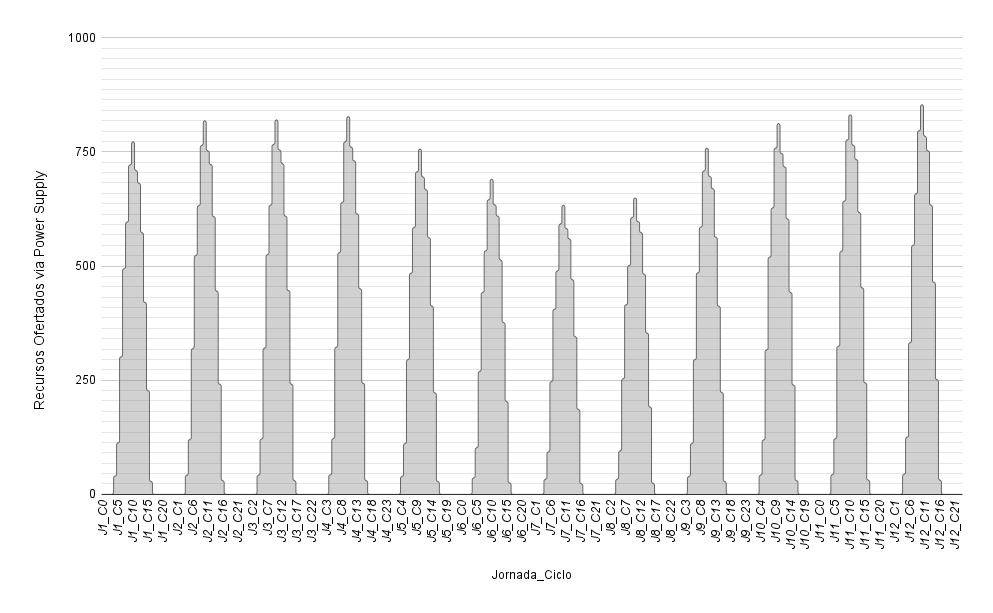
\includegraphics[width=1\linewidth]{Imagens/cap6/cap6valoresofertados.png} 
	
	Fonte: elaborado pelo autor.
\end{figure}

Dada a natureza do experimento, qualquer execução obterá o mesmo comportamento e distribuição para seus valores ofertados, pois são definidos antes da execução e não sofrem impacto diante das caracteristicas dos dispositivos dentro do contexto de uma ou outra execução.

A segunda variável independente utilizada, representa as solicitações disparadas contra a interface do dispositivo provedor. Este estimulo tem características tais que, ao atender-las, o provedor intensifica seu consumo energético, pois encontra-se em estado ativo, demandando mais recursos. Isso implica que, à medida que a quantidade das solicitações atendidas aumenta, o consumo de energia do provedor também aumentará proporcionalmente, resultando em um impacto significativo na disponibilidade do dispositivo em relação com seu desempenho energético. A Tabela \ref{table:cap6:execucaocaracteristicas}, apresenta os valores utilizados para as requisições em cada execução do experimento. A precisão indica a distribuição da relação entre total de solicitações em cada execução em referencia para 12 jornadas (8640 solicitações) descrito na Seção \ref{cap6:execucao}

\begingroup

\begin{table}[h]
	
	\centering
	\caption{Solicitaçoes realizadas}
	\begin{threeparttable}
	\begin{tabular}{ l c c c c }
		\toprule
		&   & \multicolumn{3}{c}{Solicitações}\\\cline{3-5} & Duração&
		\begin{tabular}{@{}c@{}} Exec 1\end{tabular} & \begin{tabular}{@{}c@{}} Exec 2\end{tabular} & \begin{tabular}{@{}c@{}} Exec 3\end{tabular}\\
		\bottomrule
		1 ciclo  				& 6 $seg$ 	& 29,875 	& 29,86 & 29,88 \\
		1 Jornada (24 ciclos)  	& 144 $seg$	& 717 & 716,75 &  717,16\\
		12 Jornadas  			& 1728 $seg$& 8604  & 8601 & 8606 \\
		\bottomrule
	\end{tabular}

	\end{threeparttable}
	\label{table:cap6:execucaocaracteristicas}
	\\
	\footnotesize Fonte: elaborado pelo autor.
	
\end{table}
\endgroup


Dando prosseguimento à execução do experimento, as variáveis dependentes são obtidas para avaliação: A Quantidade total de solicitações atendidas ao fim da execução do experimento e a evolução desses valores; a quantidade de solicitações impedidas mediante indisponibilidade do dispositivo. Para analisar a quantidade de solicitações impedidas, é preciso contrapor os dados temporais da variável independente oferta energética em relação a quantidade presente no dispositivo, o que justificará a atuação de limitadores.

Ainda sobre os dados coletados, ao final de cada execução foi coletado o total de requisições atendidas por cada dispositivo. Conforme Figura \ref{fig:cap6solicitacoesatendidas}, é possível comparar o desempenho dos dispositivos sob a ponto de vista das solicitações atendidas.

\begin{figure}[H]
	\centering	
	\caption{Quantidade de solicitações atendidas por dispositivo.} 
	\label{fig:cap6solicitacoesatendidas}
	\noindent\includegraphics[width=0.8\linewidth]{Imagens/cap6/cap6solicitaçoesatendidas_execs.png} 
	
	Fonte: elaborado pelo autor.
\end{figure}

Apenas o dispositivo "no-throttling" apresentou-se como resultado um quadro de indisponibilidade em função de esgotamento energético, de modo geral a Tabela \ref{table:cap6:quadrogeralobtido} apresenta a performance dos dispositivos para atender as solicitações e quando necessário apresentar o quadro de indisponibilidade em razão do total de solicitações realizadas.

\begingroup
\begin{table}[H]
	\centering
	\caption{Quadro das solicitações realizadas aos dispositivos}
	\begin{tabular}{|c |c |c|c|c|}
		\hline
		\multirow{2}{*}{Execução} & 
		\multirow{2}{*}{Dispositivo} &
		\multicolumn{2}{c|}{Solicitações} & 
		\multirow{2}{*}{\% indisponíveis} \\
		& & atendidas & indisponíveis & \\
		\midrule
		1& 	no-throttling 	&  7043&1561 & 0.1814\\
		1& 	fixed-throttling &  3414&0 & -\\
		1&	dynamic-throttling & 5098 & 0 &-\\
		
		2& no-throttling &  7105&1496 & 0.1739\\
		2& fixed-throttling & 3436& 0 & -\\
		2& dynamic-throttling & 5118& 0 &-\\
		
	   3  &	no-throttling & 7105& 1504& 0.1747\\
	   3	& fixed-throttling &3441 & 0& -\\
	   3	& dynamic-throttling & 5123& 0&-\\
		
		\bottomrule
	\end{tabular}
		\label{table:cap6:quadrogeralobtido}
		\\
		\footnotesize Fonte: elaborado pelo autor.
\end{table}
\endgroup

Parte da análise é obtida ao observar o gráfico de comportamento referente às capacidades energéticas encontradas no \textit{storage} do dispositivo. A Figura \ref{fig:cap6recortecomportamentostorage} apresenta um recorte dos dados, oferecendo informações suficientes para analisar a dinâmica entre a coleta e o consumo de recursos realizada por todos os dispositivos envolvidos. Essa visualização permite identificar padrões de consumo e tendências de eficiência especialmente nas áreas destacadas onde a quantidade de recurso disponibilizado é mínima.

\begin{figure}[H]
	\centering	
	\caption{Recorte do comportamento de uso dos recursos durante Execução 3.} 
	\label{fig:cap6recortecomportamentostorage}
	\noindent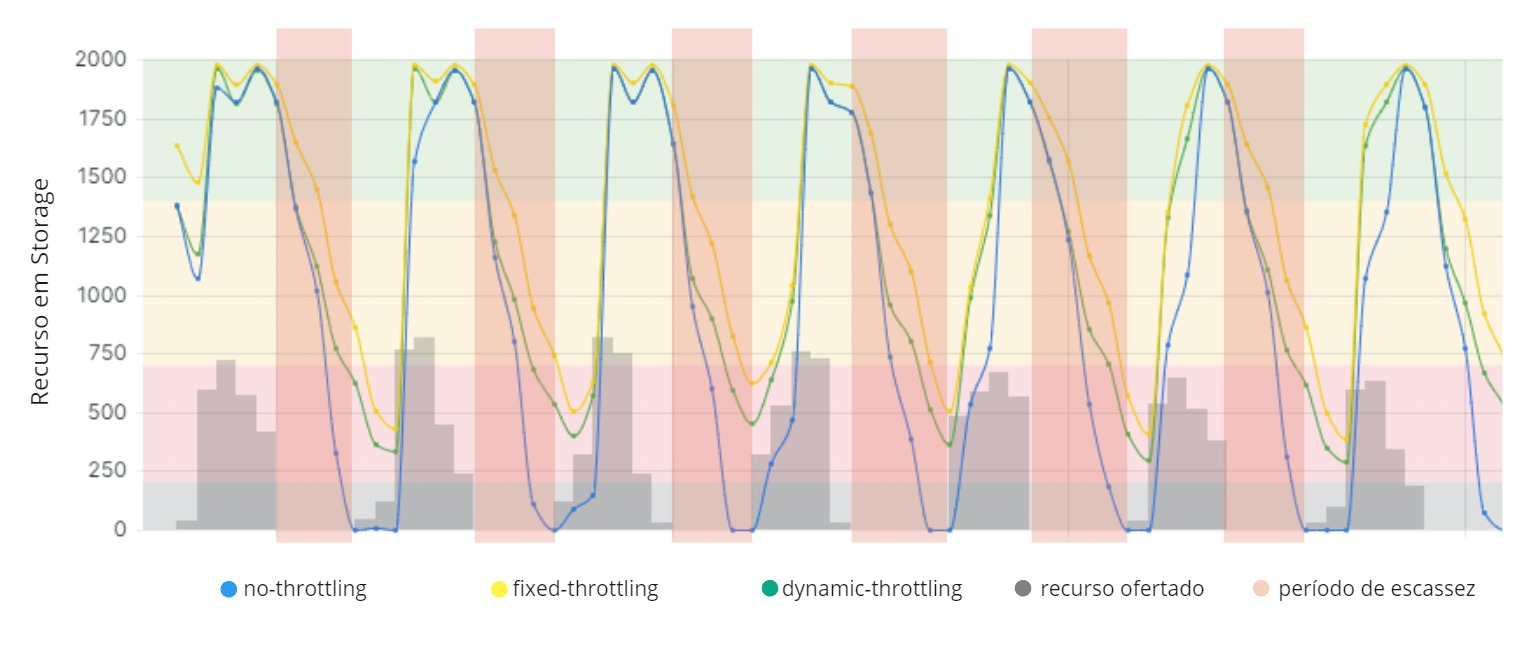
\includegraphics[width=1\linewidth]{Imagens/cap6/cap6recortecomportamentostorage.jpg} 
	
	Fonte: elaborado pelo autor.
\end{figure}

Ainda sobre a Figura \ref{fig:cap6recortecomportamentostorage}, ela permite a análise do comportamento do dispositivo \textit{dynamic-throttling} enquanto a atuação é adaptada para cada modo de operação em referencia a sua condição apresentada em \textit{storage}, este processo é notável através da variação na tendencia da linha de consumo enquanto alterna-se as faixas horizontais limitadas pela relação de cores e modos da seguinte forma:

\begin{itemize}
	\item Verde : Modo Abundante.
	\item Amarelo : Modo Atenção.
	\item Vermelho : Modo Alerta.
	\item Cinza : Modo Hibernação.
\end{itemize} 

\subsection{Interpretação dos Resultados}
\begin{comment}
	Descreva os resultados dos testes de uma maneira que seja compreensível para o leitor. Discuta se os resultados foram estatisticamente significativos e o que isso significa em termos do seu experimento.
\end{comment}

\subsection{Limitações do Estudo}
\begin{comment}
	Reconheça quaisquer limitações do seu estudo que possam ter afetado os resultados. Isso pode incluir limitações metodológicas, questões de amostragem, viéses potenciais ou qualquer outra consideração importante.
\end{comment}




 